\begin{abstract}
Η συγκεκριμένη διπλωματική ε\-ργα\-σία έχει στόχο την επίτευξη 
υπολογισμού της θέσης - στον τρισδιάστατο χώρο - ενός πρότυπου α\-ντι\-κειμένου, 
από ένα σμήνος drone\udot με όσο δυνατόν χαμηλότερο κόστος υλικού ανά node του 
συστήματος. Ιδανικά θα γίνει προσπάθεια να γίνει multi sensor data fusion 
και να αξιοποιηθούν πληροφορίες τόσο με βάση image-based τεχνικών υπολογισμού, 
όπως επίσης και RF-based.
\end{abstract}
  
\begin{keywords}
Drone, UAV, Swarm, OpenCV, Robot Operating System, Camera, Ultra-Wideband
\end{keywords}
%%%%%%%%%%%%%%%%%%%%%%%%%%%%%%%%%%%%%%%%%%%%%%%%%%%%%%%%%%%%%%%%%%%%%%%%%%%%%%%%

\section{INTRODUCTION}
Τα τελευταία χρόνια ο χώρος των αεροχημάτων παρουσιάζει αρκετά μεγάλο ερευνητικό 
ενδιαφέρον, με αποτέλεσμα την εμφάνιση σμηνών από drone σε ένα μεγάλο
πλήθος εφαρμογών. 

Σε αυτού του τύπου τις εφαρμογές είναι πολύ σημαντική η γνώση της θέσης του κάθε 
μεμονωμένου Unmanned Aerial Vehicle (UAV) είτε σχετικά με τα γειτονικά nodes του 
συστήματος, είτε σε συ\-νδυα\-σμό αυτού και κατά απόλυτο τρόπο\udot σύμφωνα με ένα 
καθορισμένο σύστημα αξόνων.

Παρόλο, την πολλά υποσχόμενη, εξέλιξη της ακρίβειας από $\sim$5m \cite{gps-accuracy}
σε $\sim$30cm \cite{superaccurate-gps} - για μη στρατιωτική χρήση - των 
Global Navigation Satellite System (GNSS)\udot
όπου όμως ούτε αυτή δεν είναι αρκετή για τις ανάγκες ορισμένων εφαρμογών, 
πολλές φορές οδηγούμαστε ή να κινηθούμε σε αρκετά ακριβές 
λύσεις - όπως τα RTK GPS \cite{rtk-gps}, που μπορούν να προσφέρουν ακρίβεια 1-2cm σε 
ακτίνες $\sim$20km - ή να αναζητήσουμε άλλους τρόπους υπολογισμού της θέσης
των drone σε ένα swarm.

Στην υφιστάμενη βιβλιογραφία, μπορεί κανείς εύκολα να βρει μεθόδους ανεύρεση της θέσης  
των drones με τεχνικές (Remote Frequency) RF, όπως μέτρηση απόστασης με 
χρήση Ultra-Wideband (UWB) \cite{ultra-wide-band-localization}, με χρήση Infrared and Ultrasonic \cite{infrared-and-ultrasonic-localization}, 
είτε ακόμα και με την βοήθεια καμερών \cite{camera-localization}. Ενώ επίσης, πολλές φορές είναι
εξίσου σημαντικό εκτός από τον υπολογισμός της θέσης των ίδιων των drone\udot να βρούμε και την
θέση επιπλέον αντικειμένων τα οποία σχετίζονται με την εκάστοτε εφαρμογή.

\section{THESIS STATEMENT}
Όταν αναφερόμαστε σε motion capturing systems \cite{motion-capture}, όπως το Vicon \cite{vicon} 
ή το Optitrack \cite{optitrack}, μιλάμε κυρίως για στατικά, εσωτερικών χώρων συστήματα 
τα οποία είναι υπεύθυνα να ανιχνεύουν και να συλλαμβάνουν την κίνηση σωμάτων.

Στην συγκεκριμένη διπλωματική εργασία θα γίνει μία πρώτη προ\-σπά\-θεια επίλυσης του 
προβλήματος υπο\-λο\-γι\-σμού της θέσης ενός μεμονωμένου - γνωστών διαστάσεων - αντικειμένου 
με χρήση drones swarm που πραγματοποιεί close formation flight, όπως παρουσιάζεται στο Figure \ref{fig:1} με σκοπό μελλοντικά να χρησιμοποιηθούν ως feature points και 
να είμαστε πιο κοντά σε ένα real time tra\-cking σύστημα αντικειμένων για εξωτερικούς χώρους και δυναμικά περιβάλλοντα.


\begin{figure}[thpb]
  \centering
  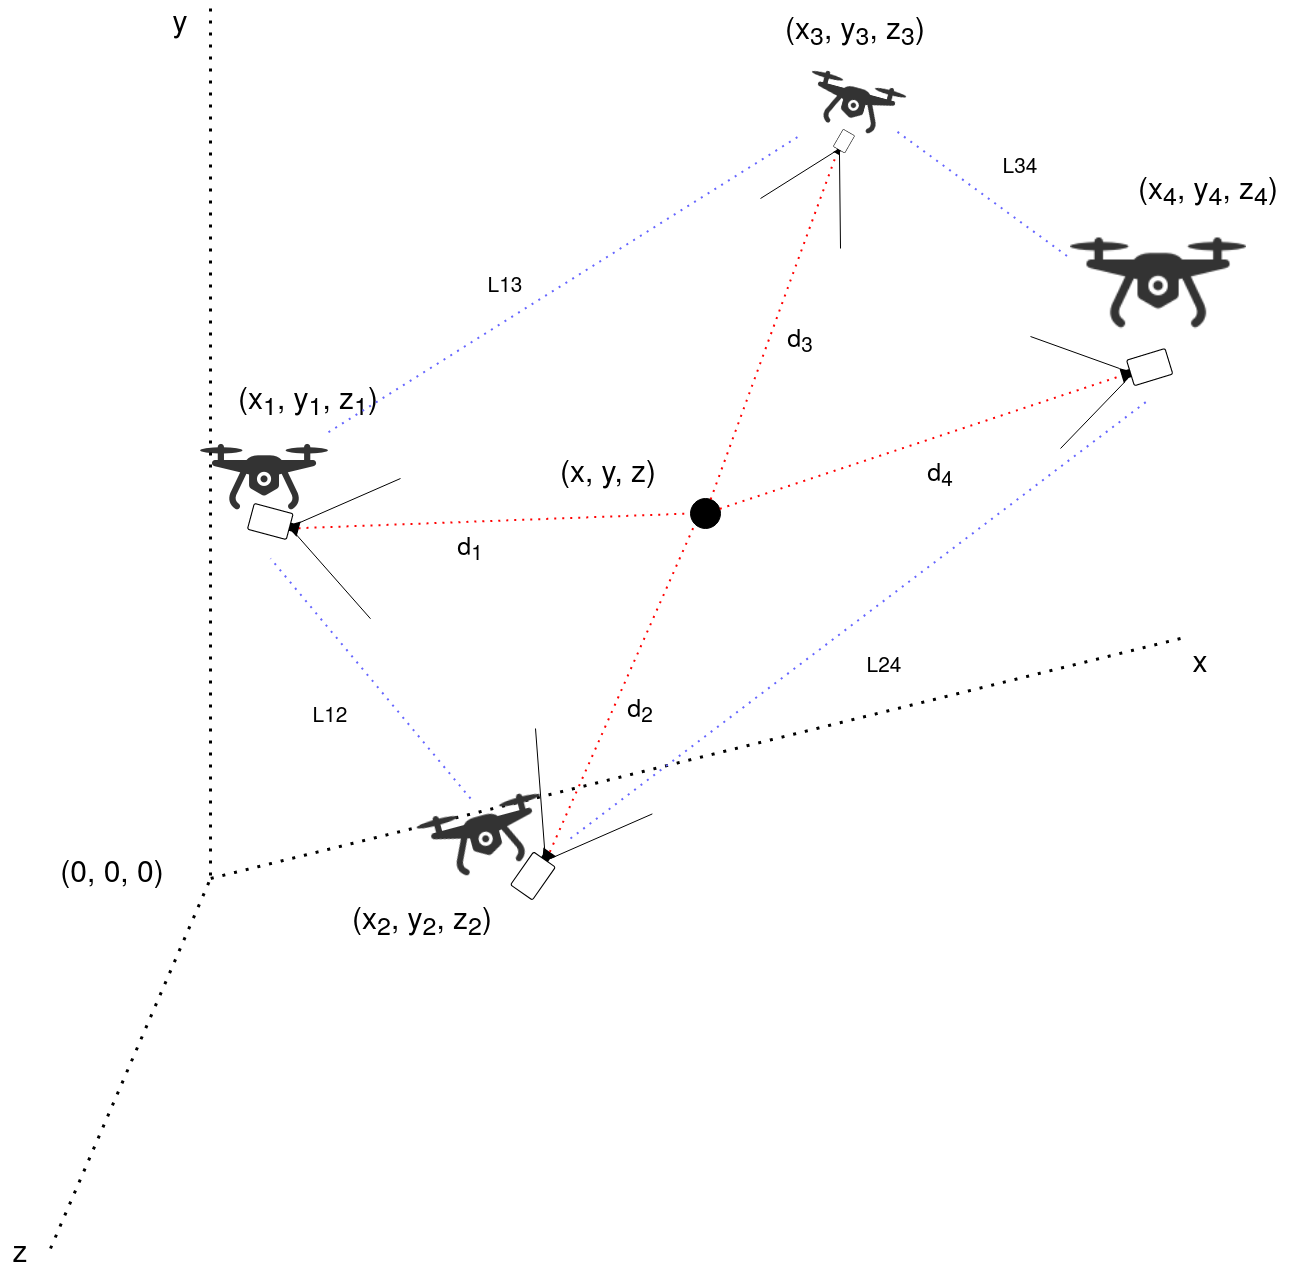
\includegraphics[width=\linewidth]{Images/3dDrones-camera-pose.png}
  \caption{Drones track object in 3D space}
  \label{fig:1}
\end{figure}

\section{APPROACH}
Ο τρόπος με τον οποίο θα γίνει προσπάθεια να λυθεί το συγκεκριμένο πρόβλημα, είναι αρχικά με χρήση monocular
vision να εντοπιστεί το αντικείμενο στο χώρο, να απομονωθεί μόνο χρήσιμη πληροφορία για αυτό   
- όπως φαίνεται στο Figure \ref{fig:2} - και στην συνέχεια με βάση την γνώση των ακριβών του διαστάσεων,
καθώς επίσης και το πλήθος των pixel που καταλαμβάνει στην κάμερα\udot να υπολογιστεί η απόσταση που 
έχει το αντικείμενο από αυτήν. 

Στην συνέχεια, για κάθε drone να ληφθούν πληροφορίες της θέσης του - μέσω GPS, IMU, κλπ αισθητήρων -
και αφού έχει γίνει το κατάλληλο φιλτράρισμα των πληροφοριών, να ομαδοποιηθούν όλες οι πληροφορίες και 
να αποσταλούν στα γειτονικά drones του συστήματος. 

Αφού πλέον το κάθε drone λάβει από τα γειτονικά τις 
θέσεις των υπόλοιπων καθώς και την απόσταση του αντικειμένου από αυτά, μπορεί να γίνει χρήση κατάλληλου
cooperative and range based localization algorithm προκειμένου να υπολογιστούν οι συντεταγμένες του αντικειμένου.
Κύριο σημείο ενδια\-φέ\-ρο\-ντος είναι αρχικά να επιτευχθεί relative positioning του α\-ντι\-κει\-μένου με real time 
onboard sensing and computing χωρίς αναγκαστικά την ύπαρξη ενός εξωτερικού infrastructure.

\begin{figure}[thpb]
  \centering
  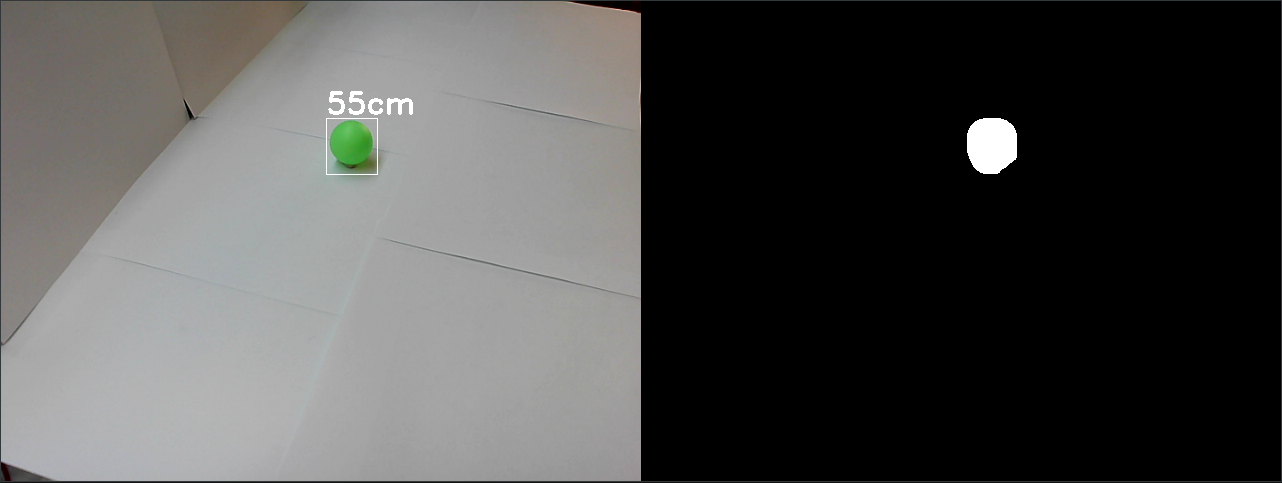
\includegraphics[width=\linewidth]{Images/Thesis-Proposal-shape-color-detection.png}
  \caption{Blob detection - σύμφωνα με το σχήμα/χρώμα - της μπάλας και υπολογισμός της απόστασης της από την κάμερα}
  \label{fig:2}
\end{figure}

\section{HARDWARE SETUP AND IMPLEMENTATION}
Σκοπός είναι όλη η επεξεργασία να πραγματοποιηθεί σε κάποιο Embedded Linux System. 
Λόγω των αρχικών πε\-ριο\-ρι\-σμών επίσκεψης του εργαστηρίου MHL (που σχετίζονται σχετικά με την πανδημία COVID-19)
η αρχική ανάπτυξη του συστήματος ξεκίνησε πάνω σε Raspberry pi 4 - Table \ref{tab:1} - ενώ στην συνέχεια αν κριθεί απαραίτητο
θα γίνει migration ενός ή περι\-σσό\-τε\-ρων nodes του συστήματος σε κάποια πλακέτα Jetson - δίνεται για παράδειγμα 
στο Table \ref{tab:2} ένα από τα συστήματα της οικογένειας Jetson - τα οποία μπορούν να προσφέρουν μεγαλύτερες ικανότητες
επεξεργασίας εικόνας. 

Σημαντικό είναι ακόμα, η χρήση 1080p κάμερας για καλύτερα αποτελέσματα λόγω ανάλυσης, αλλά παρόλα αυτά εάν χρειαστεί να 
υπάρχουν επίσης δυνατότητες downscaling. 

Τέλος, θα χρησιμοποιηθούν drone του εργαστηρίου Senselab εάν χρειαστεί να πραγματοποιηθούν πραγματικές πτήσεις με drone στο στάδιο του testing,
βάση των οποίων θα γίνει και ο σχεδιασμός των περιορισμών του συστήματος (μέγιστο payload και ισχύ που μπορούν να προσφέρουν). 

Σχετικά με το κομμάτι του software, η υλοποίηση θα πε\-ρι\-λα\-μβάνει κυρίως κώδικες σε C++, πιθανόν Python και Bash scripting.

\begin{table}[H]
  \caption[]{Raspberry Pi 4 Model B Specifications}
  \label{tab:1}
  \centering
  \begin{tabular}{ll}
      \hline
      \textbf{Feature} & \textbf{Value}  \\
      \hline
          Processor & \Centerstack{Broadcom BCM2711, Quad core Cortex-A72 \\(ARM v8) 64-bit SoC @ 1.5GHz }\\
          Memory & 8GB LPDDR4-3200 SDRAM \\
          Storage & External Micro-SD \\  
          Power & 5V DC (maximum 3A), 5-15Watt \\
          Cost & $\sim$100 €\\
          Weight & 46 grams (without case), 99 grams (with case) \\
          Peripherals & GPIO, I2C, SPI, UART \\
          \hline
  \end{tabular}
\end{table}


\begin{table}[H]
  \caption[]{Jetson Nano Developer Kit Specifications}
  \label{tab:2}
  \centering
  \begin{tabular}{ll}
      \hline
      \textbf{Feature} & \textbf{Value}  \\
      \hline
          CPU & Quad-core ARM Cortex-A57 MPCore processor\\
          GPU & \Centerstack{NVIDIA Maxwell architecture with 128 NVIDIA\\ CUDA® cores} \\
          Memory & 4 GB 64-bit LPDDR4; 25.6 gigabytes/second \\
          Storage & External Micro-SD \\  
          Power & 5V DC, 5-10Watt \\
          Cost & $\sim$120€\\
          Weight & 250 grams (without case)\\
          Peripherals & GPIO, I2C, I2S, SPI, UART \\
          \hline
  \end{tabular}
\end{table}

\section{WORK PLAN}
Σε πρώτο επίπεδο θα αποκτηθούν γνώσεις σχετικά με την βιβλιοθήκη OpenCV \cite{opencv}, μέσω της οποίας
με οπτικό τρόπο θα εντοπιστεί το αντικείμενο για τον υπολογισμό της απόστασης του από την
κάμερα.

Στην συνέχεια θα αποκτηθούν γνώσεις σχετικά με το framework Robot Operating System (ROS) \cite{ros} το οποίο 
πε\-ρι\-λα\-μβά\-νει ένα εκτενές σύνολο εργαλείων, βιβλιοθηκών και συ\-μβά\-σεων. Τα πακέτα του οποίου θα χρησιμοποιηθούν για την
λήψη και φιλτράρισμα από τους αισθητήρες των πληροφοριών, επικοινωνία μεταξύ των drone όπως τέλος και 
όποια τρι\-σδιά\-στα\-τη απεικόνιση χρειαστεί. 

Αφού έχουν συλλεχθεί οι πληροφορίες, έμφαση θα δοθεί στην επιλογή κατάλληλου cooperative and range based localization algorithm.

Τέλος, σε πε\-ρί\-πτωση όπου επι\-τρα\-πεί χρο\-νικά θα γίνει προ\-σπά\-θεια βελτίωσης των σφαλμάτων του 
GPS με την βοήθεια κάποιου RF-based μεθόδου (π.χ. με χρήση UWB και του προτύπου IEEE 802.15.4-2011 όπου
υπόσχεται ακρίβεια εκτίμησης απόστασης <10cm \cite{uwb-accuracy}).



